\documentclass[aspectratio=169,11pt]{beamer}
 
% ---------------------------------------------------------------- thema
\usetheme[
  progressbar=frametitle,
  numbering=fraction,
  sectionpage=progressbar,
  block=fill
]{metropolis}
 
\usepackage[T1]{fontenc}
\IfFileExists{dutch.ldf}{%
  \usepackage[dutch]{babel}%
  \AtBeginDocument{\shorthandoff{"}}
}{}
 
\IfFileExists{plex-sans.sty}{\usepackage[sfdefault]{plex-sans}}{}
\IfFileExists{plex-mono.sty}{\usepackage[scale=0.95]{plex-mono}}{}
 
\usepackage{tikz}
\usetikzlibrary{positioning}
\usepackage{listings}
 
\definecolor{kulblauw}{HTML}{1D8DB0}
\definecolor{kuldonker}{HTML}{00407A}
 
\setbeamercolor{frametitle}{bg=kuldonker, fg=white}
\setbeamercolor{progress bar}{fg=kulblauw, bg=kulblauw!20}
\setbeamercolor{alerted text}{fg=kulblauw}
\setbeamercolor{standout}{bg=kuldonker, fg=white}
\setbeamercolor{block title}{bg=kulblauw!20, fg=kuldonker}
\setbeamercolor{block body}{bg=kulblauw!6}
\setbeamercolor{block title alerted}{bg=orange!25, fg=black}
\setbeamercolor{block body alerted}{bg=orange!8}
 
% ---------------------------------------------------------------- code
\definecolor{codebg}{HTML}{EEF4F8}
\definecolor{codecomment}{HTML}{6A7A86}
\definecolor{codestring}{HTML}{2E7D32}
\definecolor{codetype}{HTML}{C2185B}   % Int, Char, ...
\definecolor{codefunc}{HTML}{4A6FD1}   % replicate, swap, ...
\definecolor{codeop}{HTML}{E5395C}     % :: -> => <-
\definecolor{codenum}{HTML}{D9730D}    % 3, 10, ...
\definecolor{codekw}{HTML}{8E44AD}     % where, let, ...

\newcommand{\hsop}[1]{{\color{codeop}#1}}
\newcommand{\hsnum}[1]{{\color{codenum}#1}}

\lstdefinestyle{hs}{
  language=Haskell,
  sensitive=true,
  % keywords
  keywords={where,let,in,import,if,then,else,case,of,data,type,module,
            newtype,class,instance,deriving},
  keywordstyle=\color{codekw}\bfseries,
  % types
  keywords=[2]{Int,Char,String,Bool,Integer,Double,Float,Maybe,Either,
               Ord,Eq,Show,Num,True,False,Just,Nothing},
  keywordstyle=[2]\color{codetype},
  % Prelude / user-defined functions
  keywords=[3]{replicate,flip,map,filter,length,zip,unzip,zipWith,span,
               break,sort,sortOn,curry,uncurry,swap,optellen,fst,snd,head,
               tail,sum,product,lines,words,unwords,read,show,foldr,foldl,
               reverse,concat,concatMap,take,drop,takeWhile,dropWhile,
               elem,all,any,maximum,minimum,abs,id,const,not},
  keywordstyle=[3]\color{codefunc},
  basicstyle=\ttfamily\footnotesize,
  commentstyle=\color{codecomment}\itshape,
  stringstyle=\color{codestring},
  backgroundcolor=\color{codebg},
  columns=fullflexible, keepspaces=true,
  showstringspaces=false, upquote=true,
  xleftmargin=6pt, xrightmargin=6pt,
  framexleftmargin=6pt, framexrightmargin=6pt,
  framextopmargin=3pt, framexbottommargin=3pt,
  frame=single, rulecolor=\color{codebg},
  aboveskip=5pt, belowskip=5pt,
  escapeinside={<@}{@>},
  literate=
    {->}{{\hsop{$\rightarrow$}}}2
    {<-}{{\hsop{$\leftarrow$}}}2
    {=>}{{\hsop{$\Rightarrow$}}}2
    {::}{{\hsop{::}}}2
    {==}{{\hsop{==}}}2
    {0}{{\hsnum{0}}}1 {1}{{\hsnum{1}}}1 {2}{{\hsnum{2}}}1
    {3}{{\hsnum{3}}}1 {4}{{\hsnum{4}}}1 {5}{{\hsnum{5}}}1
    {6}{{\hsnum{6}}}1 {7}{{\hsnum{7}}}1 {8}{{\hsnum{8}}}1
    {9}{{\hsnum{9}}}1
    {ë}{{\"e}}1 {é}{{\'e}}1 {è}{{\`e}}1,
}
\lstset{style=hs}

% inline code: same colors, plain text in dark blue
\lstdefinestyle{hsinline}{
  basicstyle=\ttfamily\color{kuldonker},
}
\newcommand{\hs}{\lstinline[style=hsinline]}
 
% ---------------------------------------------------------------- titel
\title{Sessie I: Haskell de basics}
\subtitle{PAL-sessie Declaratieve Talen}
\author{Yarne Ramakers, Yendric Van Roey}
\institute{KU Leuven}
\date{\today}
 
\begin{document}
 
\maketitle

\begin{frame}[standout]
  Zijn er vragen vanuit de oefenzittingen?
\end{frame}

\begin{frame}{Planning voor vandaag}
  \begin{enumerate}
    \item \textbf{Nuttige functies uit de standard library}
      \begin{itemize}
        \item even opfrissen: \hs|.|, \hs|$| en \hs|flip|
        \item \hs|curry| en \hs|uncurry|
        \item \hs|swap|
        \item \hs|zip|, \hs|unzip| en \hs|zipWith|
        \item \hs|span| en \hs|break|
        \item \hs|sort| en \hs|sortOn|
        \item documentatie zoeken en \hs|hlint|
      \end{itemize}
    \item \textbf{Lazy evaluation}
    \item \textbf{Hlint}
    \item \textbf{Opdrachten}
  \end{enumerate}
\end{frame}

\section{Nuttige functies uit de Prelude}
 
\begin{frame}[fragile]{Even opfrissen: \texttt{.}, \texttt{\$} en \texttt{flip}}
\begin{lstlisting}
(.)  :: (b -> c) -> (a -> b) -> a -> c        (f . g) x  =  f (g x)
($)  :: (a -> b) -> a -> b                    f $ x      =  f x
flip :: (a -> b -> c) -> b -> a -> c          flip f x y =  f y x
\end{lstlisting}
  \hs|$| heeft de \alert{laagste prioriteit} en bespaart je zo haakjes. Drie keer hetzelfde:
\begin{lstlisting}
length (filter (> 3) (map (* 2) xs))
length $ filter (> 3) $ map (* 2) xs
(length . filter (> 3) . map (* 2)) xs
\end{lstlisting}
  \hs|flip| wisselt de eerste twee argumenten om:
\begin{lstlisting}
flip replicate 'a' 3 == "aaa"
\end{lstlisting}
\end{frame}

\begin{frame}[fragile]{Kleine quiz}
  Gegeven:
\begin{lstlisting}
zipWith :: (a -> b -> c) -> [a] -> [b] -> [c]
flip    :: (x -> y -> z) -> y -> x -> z
\end{lstlisting}
  Wat is het type van \hs|flip zipWith|?

  \bigskip
  \begin{itemize}
    \item[\textbf{A}] \hs|(b -> a -> c) -> [a] -> [b] -> [c]|
    \medskip
    \item[\textbf{B}] \hs|(a -> b -> c) -> [b] -> [a] -> [c]|
    \medskip
    \item[\textbf{C}] \hs|[a] -> (a -> b -> c) -> [b] -> [c]|
    \medskip
    \item[\textbf{D}] \hs|[c] -> [b] -> [a] -> (a -> b -> c)|
  \end{itemize}
\end{frame}

\begin{frame}[fragile]{Kleine quiz: antwoord \textbf{C}}
  Elke functie neemt maar \alert{één} argument, dus lees \hs|zipWith| als:
\begin{lstlisting}
zipWith :: (a -> b -> c) -> ([a] -> ([b] -> [c]))
           -------------    ---    ------------
                 x           y          z
\end{lstlisting}
  \hs|flip| wisselt \alert{enkel de eerste twee} argumenten om; de rest (\hs|z|) blijft staan:
\begin{lstlisting}
flip zipWith :: [a] -> (a -> b -> c) -> [b] -> [c]

flip zipWith [1, 2, 3] (+) [10, 20, 30]  == [11, 22, 33]
\end{lstlisting}
  \pause
  \small
  \begin{tabular}{@{}l l@{}}
    \textbf{A} & wisselt de argumenten van de functie \alert{binnenin}: dat doet \hs|flip| niet \\
    \textbf{B} & wisselt de \alert{laatste} twee argumenten, maar \hs|flip| pakt de eerste twee \\
    \textbf{D} & draait het \alert{hele} type om; het resultaat blijft \hs|[c]| \\
  \end{tabular}
\end{frame}

\begin{frame}[fragile]{Elke functie neemt maar één argument}
  De pijl \hs|->| is rechts-associatief. Deze twee types zijn dus \alert{hetzelfde}
  \begin{lstlisting}
replicate :: Int -> a -> [a]
replicate :: Int -> (a -> [a])
\end{lstlisting}
  Je kan ook maar een deel van de argumenten geven (\alert{partiële toepassing}):
  \begin{lstlisting}
replicate 3      :: a -> [a]        -- een nieuwe functie!
replicate 3 'x'  :: [Char]          -- "xxx"
\end{lstlisting}
  Soms zitten de argumenten echter samen in een \alert{koppel}:
  \begin{lstlisting}
optellen :: (Int, Int) -> Int       -- maar één argument: een tuple
optellen (x, y) = x + y             -- hoe zet je de ene vorm om in de andere?
\end{lstlisting}
\end{frame}

\begin{frame}[fragile]{\texttt{curry} en \texttt{uncurry}}
  \begin{center}
  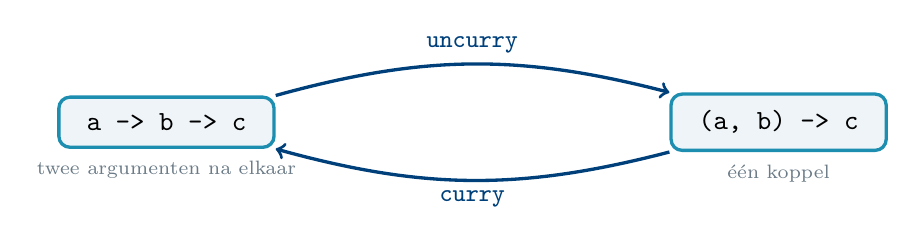
\begin{tikzpicture}[
      box/.style={draw=kulblauw, very thick, rounded corners, fill=codebg,
                  inner xsep=10pt, inner ysep=6pt, font=\ttfamily}]
    \node[box] (c) {a -> b -> c};
    \node[box, right=5cm of c] (u) {(a, b) -> c};
    \draw[->, very thick, kuldonker] (c.north east) to[bend left=15]
      node[above, font=\ttfamily\small]{uncurry} (u.north west);
    \draw[->, very thick, kuldonker] (u.south west) to[bend left=15]
      node[below, font=\ttfamily\small]{curry} (c.south east);
    \node[below=1pt of c, font=\scriptsize, text=codecomment] {twee argumenten na elkaar};
    \node[below=1pt of u, font=\scriptsize, text=codecomment] {één koppel};
  \end{tikzpicture}
  \end{center}
  \vspace{-4pt}
\begin{lstlisting}
uncurry :: (a -> b -> c) -> ((a, b) -> c)       uncurry f (x, y) = f x y
curry   :: ((a, b) -> c) -> (a -> b -> c)       curry f x y      = f (x, y)
\end{lstlisting}
  Bijvoorbeeld:
\begin{lstlisting}
uncurry replicate :: (Int, a) -> [a]
curry optellen    :: Int -> Int -> Int
\end{lstlisting}
\end{frame}

\begin{frame}[fragile]{Kleine quiz: \texttt{curry} en \texttt{uncurry}}
  Wat is het resultaat?
  \begin{onlyenv}<1>
  \begin{lstlisting}
uncurry replicate (3, 'x')                       -- ?
curry fst 'a' True                               -- ?
map (uncurry (++)) [("ab", "c"), ("", "de")]     -- ?
\end{lstlisting}
\end{onlyenv}
\begin{onlyenv}<2->
\begin{lstlisting}
uncurry replicate (3, 'x')                       -- "xxx"
curry fst 'a' True                               -- 'a'
map (uncurry (++)) [("ab", "c"), ("", "de")]     -- ["abc", "de"]
\end{lstlisting}
\end{onlyenv}
  \medskip
  En wat is het \alert{type} van \hs|uncurry (++)|?
\begin{uncoverenv}<3->
\begin{lstlisting}
uncurry (++) :: ([a], [a]) -> [a]
\end{lstlisting}
\end{uncoverenv}
\end{frame}

\begin{frame}[fragile]{Swap en tuples}
  \hs|swap| wisselt de twee elementen van een \alert{koppel} om.\\
  Zit niet in de Prelude! \hs|import Data.Tuple (swap)|

\begin{lstlisting}
swap :: (a, b) -> (b, a)
swap (x, y) = (y, x)
\end{lstlisting}
\begin{lstlisting}
swap (1, "een") == ("een", 1)
map swap [(1, 'a'), (2, 'b')] == [('a', 1), ('b', 2)]
\end{lstlisting}
\pause
\hs|swap| werkt op een \alert{koppel}, \hs|flip| op de \alert{argumenten van een functie}.
Met \hs|curry| en \hs|uncurry| zie je het verband:
\begin{lstlisting}
curry swap :: a -> b -> (b, a)          -- curry swap 1 'x' == ('x', 1)
uncurry (flip replicate) ('z', 3)  ==  uncurry replicate (swap ('z', 3))
\end{lstlisting}
\end{frame}

\begin{frame}[fragile]{\texttt{flip} en \texttt{swap}: twee kanten van hetzelfde idee}
Met \hs|curry| en \hs|uncurry| kan je de ene uitdrukken in de andere:
\begin{lstlisting}
flip' :: (a -> b -> c) -> b -> a -> c
<@\onslide<2->@>flip' f = curry (uncurry f . swap)<@\onslide@>

swap' :: (a, b) -> (b, a)
<@\onslide<3->@>swap' = uncurry (flip (,))          -- (,) :: a -> b -> (a, b)  =  curry id<@\onslide@>
\end{lstlisting}
\onslide<4->
\begin{columns}[T,onlytextwidth]
    \begin{column}{0.49\textwidth}
\begin{lstlisting}
  flip' f x y
= curry (uncurry f . swap) x y
= (uncurry f . swap) (x, y)
= uncurry f (swap (x, y))
= uncurry f (y, x)
= f y x
\end{lstlisting}
    \end{column}
    \onslide<4->
    \begin{column}{0.49\textwidth}
\begin{lstlisting}
  swap' (x, y)
= uncurry (flip (,)) (x, y)
= flip (,) x y
= (,) y x
= (y, x)
\end{lstlisting}
    \end{column}
\end{columns}
\end{frame}
\begin{frame}[fragile]{\texttt{zip}}
  \hs|zip :: [a] -> [b] -> [(a, b)]| koppelt twee lijsten element per element.
  Het stopt bij de \alert{kortste} lijst:
\begin{lstlisting}[aboveskip=2pt]
zip :: [a] -> [b] -> [(a, b)]
zip (x : xs) (y : ys) = (x, y) : zip xs ys
zip _        _        = []

zip [1, 2, 4] ['a', 'b', 'd']  == [(1, 'a'), (2, 'b'), (4, 'd')]
zip [1, 2, 3] "ab"             == [(1, 'a'), (2, 'b')]
\end{lstlisting}
  Daardoor mag één van de lijsten zelfs oneindig zijn:
\begin{lstlisting}
enumerate :: [a] -> [(Int, a)]
enumerate xs = zip [0 ..] xs

enumerate "Hoi" == [(0, 'H'), (1, 'o'), (2, 'i')]
\end{lstlisting}
\end{frame}

\begin{frame}[fragile]{\texttt{unzip} en \texttt{zipWith}}
  \hs|unzip :: [(a, b)] -> ([a], [b])| doet precies het omgekeerde van \hs|zip|:
\begin{lstlisting}
unzip [(1, 'I'), (5, 'V'), (10, 'X')] == ([1, 5, 10], "IVX")
\end{lstlisting}
  Met \hs|zipWith| kies je zelf wat je met de twee elementen doet:
\begin{lstlisting}
zipWith :: (a -> b -> c) -> [a] -> [b] -> [c]
zipWith (+)       [1, 2, 3] [10, 20, 30]  == [11, 22, 33]
zipWith replicate [1, 2, 3] "abc"         == ["a", "bb", "ccc"]
\end{lstlisting}
  \hs|zip| is dus een speciaal geval van \hs|zipWith|:
\begin{lstlisting}
zip xs ys == zipWith (,) xs ys
\end{lstlisting}
\end{frame}


\begin{frame}[fragile]{\texttt{span} en \texttt{break}}
  Beide hebben hetzelfde type: \hs|(a -> Bool) -> [a] -> ([a], [a])|
  
  Werking:
\begin{lstlisting}
span p xs = (takeWhile p xs, dropWhile p xs) -- zolang p waar is in eerste,
                                             -- alles erachter in tweede
break p = span (not . p)                     -- tegengestelde van span
\end{lstlisting}
Voorbeeld (lijst splitsen):
\begin{lstlisting}
span (<= 3) [1..6] == ([1, 2, 3], [4, 5, 6])
span (<= 3) [1, 2, 3, 4, 3] == ([1, 2, 3], [4, 3]) -- tweede drie komt rechts
break (== ' ') "hello world yendric"  ==  ("hello", " world yendric")
\end{lstlisting}
\end{frame}

\begin{frame}[fragile]{\texttt{sort} en \texttt{sortOn}}
Dienen geïmporteerd te worden: 
\begin{lstlisting}
import Data.List (sort, sortOn)
\end{lstlisting}
Werking:
\begin{lstlisting}
sort :: Ord a => [a] -> [a]               -- sorteert een lijst
sortOn :: Ord b => (a -> b) -> [a] -> [a] -- sorteer originele waardes op basis van 
                                 -- gemapte waardes
\end{lstlisting}
Voorbeeld:
\begin{lstlisting}
sort [('C', 0), ('A', 2), ('B', 1)] == [('A', 2), ('B', 1), ('C', 0)]
sortOn snd [('C', 0), ('A', 2), ('B', 1)] == [('C', 0), ('B', 1), ('A', 2)]
\end{lstlisting}
\end{frame}

\section{Lazy evaluation}

\begin{frame}[fragile]{Lazy evaluation: pas rekenen als het moet}
  Haskell rekent een expressie pas uit wanneer het resultaat \alert{echt nodig} is. Tot dan is het een \alert{thunk}: een uitgestelde berekening. \hs|undefined| crasht zodra je hem uitrekent, maar hier gebeurt dat nooit:
  \begin{lstlisting}[aboveskip=2pt]
fst (1, undefined)  == 1        length [undefined, undefined]  == 2
\end{lstlisting}
\pause
Wat gebeurt er bij \hs|head (map (*2) [1..])|?
\begin{lstlisting}[aboveskip=2pt]
  head (map (* 2) [1 ..])
= head (map (* 2) (1 : [2 ..]))
= head (1 * 2 : map (* 2) [2 ..])     -- de staart blijft een thunk
= 1 * 2
= 2                                   -- maar één element uitgerekend!
\end{lstlisting}
\end{frame}

\begin{frame}[fragile]{Thunks bekijken in GHCi}
  Met \hs|:sprint| toont GHCi een waarde \alert{zonder} ze uit te rekenen. Een \hs|_| is een thunk.
  \begin{columns}[T,onlytextwidth]
    \begin{column}{0.49\textwidth}
\begin{lstlisting}[aboveskip=2pt]
ghci> xs = map (*2) [1..5] :: [Int]
ghci> :sprint xs
xs = _
ghci> head xs
2
ghci> :sprint xs
xs = 2 : _
ghci> length xs
5
ghci> :sprint xs
xs = [2,_,_,_,_]
\end{lstlisting}
    \end{column}
    \begin{column}{0.49\textwidth}
      \small
      \begin{itemize}
        \item \hs|head| heeft enkel het eerste element nodig
        \item \hs|length| loopt de hele \alert{structuur} af, maar rekent de elementen zelf niet uit
        \item pas na \hs|sum xs| staat er \hs|[2,4,6,8,10]|
        \item eens uitgerekend, \alert{blijft} een waarde uitgerekend
      \end{itemize}
      \medskip
      Vergeet \hs|:: [Int]| niet, anders toont \hs|:sprint| altijd \hs|_|.
    \end{column}
  \end{columns}
\end{frame}

\begin{frame}[fragile]{Een thunk in het geheugen}
  \tikzset{
    cel/.style={draw=kuldonker, thick, fill=white, minimum size=6mm, inner sep=0pt},
    thunk/.style={draw=orange!80!black, thick, dashed, fill=orange!12, rounded corners=2pt,
                  font=\ttfamily\footnotesize, inner sep=3pt, minimum height=6mm},
    waarde/.style={draw=kuldonker, thick, fill=codebg, rounded corners=2pt,
                   font=\ttfamily\footnotesize, minimum size=6mm, inner sep=2pt},
    pijl/.style={->, >=stealth, thick, kuldonker},
    punt/.style={circle, fill=kuldonker, inner sep=0pt, minimum size=3.5pt},
  }
  % (:)-cel: linkerhelft wijst naar het element, rechterhelft naar de rest van de lijst
  \newcommand{\cons}[2]{%
    \node[cel] (#1h) at (#2) {};
    \node[cel, right=0pt of #1h] (#1t) {};
    \node[font=\ttfamily\scriptsize, text=codecomment, above=1pt of #1h.north east] {(:)};
    \node[punt] at (#1h.center) {};
    \node[punt] at (#1t.center) {};
  }
  \begin{center}
  \begin{tikzpicture}
    \path[use as bounding box] (-0.4, -2.1) rectangle (13.7, 0.8);
    \node[font=\ttfamily\large] (xs) at (0, 0) {xs};

    % stap 1: nog niets uitgerekend
    \only<1>{
      \node[thunk, right=1cm of xs] (t) {map (*2) [1..5]};
      \draw[pijl] (xs) -- (t);
    }
    % stap 2: na head xs
    \only<2>{
      \cons{a}{1.5, 0}
      \draw[pijl] (xs) -- (ah.west);
      \node[waarde] (va) at (1.5, -1.6) {2};
      \draw[pijl] (ah.center) -- (va);
      \node[thunk, right=1cm of at] (t) {map (*2) [2..5]};
      \draw[pijl] (at.center) -- (t);
    }
    % stap 3 en 4: na length xs (en sum xs)
    \only<3->{
      \foreach \n/\x in {a/1.5, b/3.95, c/6.4, d/8.85, e/11.3} { \cons{\n}{\x, 0} }
      \node[waarde] (nil) at (13.35, 0) {[]};
      \draw[pijl] (xs) -- (ah.west);
      \foreach \v/\w in {a/b, b/c, c/d, d/e} { \draw[pijl] (\v t.center) -- (\w h.west); }
      \draw[pijl] (et.center) -- (nil);
      \node[waarde] (va) at (1.5, -1.6) {2};
    }
    \only<3>{
      \foreach \n/\x/\i in {b/3.95/2, c/6.4/3, d/8.85/4, e/11.3/5} {
        \node[thunk] (v\n) at (\x, -1.6) {\i*2};
      }
    }
    \only<4>{
      \foreach \n/\x/\r in {b/3.95/4, c/6.4/6, d/8.85/8, e/11.3/10} {
        \node[waarde] (v\n) at (\x, -1.6) {\r};
      }
    }
    \only<3->{ \foreach \n in {a, b, c, d, e} { \draw[pijl] (\n h.center) -- (v\n); } }
  \end{tikzpicture}
  \end{center}

  \footnotesize
  \tikz[baseline=-0.6ex]\node[thunk, font=\ttfamily\scriptsize]{1*2}; thunk
  \qquad
  \tikz[baseline=-0.6ex]\node[waarde, font=\ttfamily\scriptsize]{2}; uitgerekende waarde
  \qquad
  \tikz[baseline=-0.6ex]{\node[cel, minimum size=4mm](p){}; \node[cel, minimum size=4mm, right=0pt of p]{};}
  \hs|(:)|-cel: element en rest

  \medskip
  \normalsize
  \only<1>{\hs|xs = map (*2) [1..5]|: er is nog \alert{niets} uitgerekend, enkel een recept.\\
    \hs|:sprint xs|\quad\(\rightarrow\)\quad\hs|_|}%
  \only<2>{Na \hs|head xs|: één \hs|(:)|-cel en één waarde. De rest blijft een thunk.\\
    \hs|:sprint xs|\quad\(\rightarrow\)\quad\hs|2 : _|}%
  \only<3>{Na \hs|length xs|: de hele \alert{structuur} bestaat, de elementen zijn nog thunks.\\
    \hs|:sprint xs|\quad\(\rightarrow\)\quad\hs|[2,_,_,_,_]|}%
  \only<4>{Na \hs|sum xs|: elke thunk werd \alert{overschreven} met zijn waarde.\\
    \hs|:sprint xs|\quad\(\rightarrow\)\quad\hs|[2,4,6,8,10]|}
\end{frame}

\begin{frame}[fragile]{Sharing: een thunk wordt maar één keer uitgerekend}
  \tikzset{
    thunk/.style={draw=orange!80!black, thick, dashed, fill=orange!12, rounded corners=2pt,
                  font=\ttfamily\small, inner sep=4pt, minimum height=7mm},
    waarde/.style={draw=kuldonker, thick, fill=codebg, rounded corners=2pt,
                   font=\ttfamily\small, inner sep=4pt, minimum size=7mm},
    pijl/.style={->, >=stealth, thick, kuldonker},
  }
\begin{lstlisting}[aboveskip=2pt]
kwadraat :: Int -> Int
kwadraat x = x * x

kwadraat (1 + 2)
\end{lstlisting}
  \begin{columns}[c,onlytextwidth]
    \begin{column}{0.35\textwidth}
      \centering
      \begin{tikzpicture}
        \alt<3>{\node[waarde] (maal) at (0, 0) {9};}
               {\node[thunk] (maal) at (0, 0) {x * x};}
        \only<1>{\node[thunk] (x) at (0, -2.2) {1 + 2};}
        \only<2>{\node[waarde] (x) at (0, -2.2) {3};}
        \only<3>{\node[waarde, opacity=0.25] (x) at (0, -2.2) {3};}
        \only<-2>{
          \draw[pijl] (maal.south west) to[bend right=35] node[left, font=\ttfamily\small]{x} (x.north west);
          \draw[pijl] (maal.south east) to[bend left=35] node[right, font=\ttfamily\small]{x} (x.north east);
        }
      \end{tikzpicture}
    \end{column}
    \begin{column}{0.6\textwidth}
      \only<1>{Haskell plakt \hs|1 + 2| \alert{niet} twee keer in de body.
        Beide \hs|x|'en wijzen naar \alert{dezelfde} thunk in het geheugen.}%
      \only<2>{De eerste \hs|x| die nodig is, rekent de thunk uit en \alert{overschrijft} hem met \hs|3|.
        De tweede \hs|x| ziet dus meteen \hs|3|.}%
      \only<3>{Resultaat: \hs|9|, en \hs|1 + 2| werd maar \alert{één keer} uitgerekend.
        Niemand wijst nog naar \hs|3|, dus dat ruimt de garbage collector op.}
    \end{column}
  \end{columns}
\end{frame}

\begin{frame}[fragile]{Oneindige lijsten}
\begin{lstlisting}[aboveskip=2pt]
[1 ..]             -- 1, 2, 3, 4, ...
repeat 'x'         -- 'x', 'x', 'x', ...
iterate (* 2) 1    -- 1, 2, 4, 8, 16, ...
cycle [1, 2, 3]    -- 1, 2, 3, 1, 2, 3, ...
\end{lstlisting}
Geen probleem, zolang je maar een \alert{eindig stuk} ervan gebruikt:
\begin{lstlisting}[aboveskip=2pt]
take 6 (iterate (* 2) 1)             == [1, 2, 4, 8, 16, 32]
takeWhile (< 50) (map (^ 2) [1 ..])  == [1, 4, 9, 16, 25, 36, 49]
zip [0 ..] "Hoi"                     == [(0, 'H'), (1, 'o'), (2, 'i')]
\end{lstlisting}
\pause
\textbf{Waarom nuttig?} Je scheidt \alert{wat} je berekent van \alert{hoeveel} je ervan nodig hebt: ``alle kwadraten'' beschrijf je één keer, wie ze gebruikt beslist waar te stoppen.
\end{frame}

\begin{frame}[fragile]{Valkuilen}
Alles wat de \alert{hele} lijst nodig heeft, stopt nooit:
\begin{lstlisting}[aboveskip=2pt]
length [1 ..]       -- blijft eeuwig rekenen (onderbreek met Ctrl+C)
sum [1 ..]          -- idem, net als last, reverse, ...
\end{lstlisting}
\pause
\hs|filter| versus \hs|takeWhile|
\begin{lstlisting}[aboveskip=2pt]
takeWhile (< 10) [1 ..]   == [1, 2, 3, 4, 5, 6, 7, 8, 9]
filter    (< 10) [1 ..]   -- [1,2,3,4,5,6,7,8,9   en dan... niets meer
\end{lstlisting}
\begin{alertblock}{Waarom?}
    \hs|takeWhile| stopt bij het \alert{eerste} element dat niet voldoet. \hs|filter| weet niet
    dat er geen kleinere getallen meer komen, en blijft zoeken.
  \end{alertblock}
\end{frame}

\begin{frame}[fragile]{HLint: laat je code nakijken}
  \textbf{HLint} leest je code en stelt \alert{eenvoudigere, idiomatischere}
  alternatieven voor.
  \medskip

  Typische beginnerscode:
\begin{lstlisting}
allPositive :: [Int] -> Bool
allPositive xs = if and (map (\x -> x > 0) xs) == True then True else False
\end{lstlisting}
  \pause
\begin{lstlisting}[language={}]
$ hlint Voorbeeld.hs
Voorbeeld.hs:2:18-75: Warning: Redundant if
Voorbeeld.hs:2:21-46: Warning: Use all
Voorbeeld.hs:2:21-54: Warning: Redundant ==
Voorbeeld.hs:2:30-42: Suggestion: Avoid lambda using `infix'
4 hints
\end{lstlisting}
\end{frame}

\begin{frame}[fragile]{HLint: hints toepassen}
  Pas alle sugesties toe en je krijgt:
\begin{lstlisting}
allPositive :: [Int] -> Bool
allPositive xs = all (> 0) xs
\end{lstlisting}

\begin{lstlisting}[language={}]
$ hlint Voorbeeld.hs
Voorbeeld.hs:2:18-75: Warning: Eta reduce
1 hints
\end{lstlisting}

Pas toe en je krijgt:

\begin{lstlisting}
allPositive :: [Int] -> Bool
allPositive = all (> 0)
\end{lstlisting}
\end{frame}

\begin{frame}[standout]
  Vragen?
\end{frame}

\section{Opdracht: Advent of Code}

\begin{frame}{Hoe denkt een functionele programmeur?}
  \begin{enumerate}
    \item \textbf{Wat gaat erin, wat komt eruit?}\\
      Schrijf eerst het type van het \alert{hele} probleem, bv.\ \hs|solve :: String -> Int|.
    \item \textbf{Splits op in kleinere stappen}\\
      Schrijf enkel de \alert{signatures}, met \hs|= undefined| als body. Dat compileert al!
    \item \textbf{Vul elk stukje apart in}\\
      Elke functie is klein en apart te testen in GHCi.
    \item \textbf{Stel samen}\\
      De oplossing is een \alert{pipeline} van kleine functies, aan elkaar gehangen met \hs|.|
  \end{enumerate}
  \pause
  \begin{block}{Waarom types eerst?}
    Een type is een \alert{belofte}: zegt wat een functie doet, voor je weet hoe.
    Vaak vertelt het type je zelfs al hoe de implementatie eruit moet zien.
  \end{block}
\end{frame}

\begin{frame}[fragile]{Invoer verwerken}
  Advent of Code geeft je altijd één grote \hs|String|.
\begin{lstlisting}
lines "3   4\n1   7"     -- ["3   4", "1   7"]
words "3   4"            -- ["3", "4"]
read "42" :: Int         -- 42
\end{lstlisting}
  \pause
  \hs|read| moet weten \alert{welk type} het moet maken. Dat haalt Haskell
  uit je typesignatuur, of je schrijft het er zelf bij met \hs|:: Int|.
  \pause
  \medskip

  Het patroon dat je bijna elke dag nodig hebt:
\begin{lstlisting}
parse :: String -> [[Int]]
parse = map (map read . words) . lines
-- "1 2 3\n4 5 6"  ->  [[1,2,3],[4,5,6]]
\end{lstlisting}
\end{frame}


\begin{frame}[fragile]{Bestanden uitlezen}
Via IO monad
\begin{lstlisting}
main :: IO ()
main = do
  input <- readFile "input.txt"
  solve input
\end{lstlisting}
\end{frame}


\begin{frame}[fragile]{Historian Hysteria (AoC 2024, dag 1)}
  \begin{columns}[T,onlytextwidth]
    \begin{column}{0.55\textwidth}
      De invoer bestaat uit twee kolommen getallen.
      \begin{itemize}
        \item koppel het \alert{kleinste} getal links aan het kleinste getal rechts,
          het op één na kleinste aan het op één na kleinste, \ldots
        \item tel de afstanden tussen alle koppels op
      \end{itemize}
      \medskip
      \href{https://adventofcode.com/2024/day/1}{\texttt{adventofcode.com/2024/day/1}}
    \end{column}
    \begin{column}{0.4\textwidth}
      Invoer:
\begin{lstlisting}
3   4
1   7
5   2
\end{lstlisting}
      \pause
      {\small
      gesorteerd: \hs|[1,3,5]| en \hs|[2,4,7]|\\
      afstanden: \(1 + 1 + 2\)\par}
      \medskip
      Uitvoer: \alert{\textbf{4}}
    \end{column}
  \end{columns}
\end{frame}

\begin{frame}[fragile]{Opdracht 1: begin bij de types}
  \textbf{Stap 1:} wat gaat erin, wat komt eruit?
\begin{lstlisting}
solve :: String -> Int
\end{lstlisting}
  \begin{uncoverenv}<2->
  \textbf{Stap 2:} in welke kleinere stukken kan je dat opsplitsen?
\begin{lstlisting}
parse         :: String -> ([Int], [Int])
totalDistance :: [Int] -> [Int] -> Int
distance      :: Int -> Int -> Int
\end{lstlisting}
  \end{uncoverenv}
  \begin{uncoverenv}<3->
  \textbf{Stap 3:} zet overal \hs|= undefined|, vul de functies één voor één in
  en test elk stuk apart in GHCi. Pas op het einde stel je \hs|solve| samen.
  \end{uncoverenv}
\end{frame}
 
\begin{frame}[fragile]{Oplossing 1: invoer parsen}
\begin{lstlisting}
parse :: String -> ([Int], [Int])
parse = unzip . map (toPair . map read . words) . lines
  where toPair [x, y] = (x, y)
\end{lstlisting}
  \pause
  Lees van \alert{rechts naar links}:
\begin{lstlisting}
"3   4\n1   7\n5   2"
    -- lines
["3   4", "1   7", "5   2"]
    -- map (toPair . map read . words)
[(3,4), (1,7), (5,2)]
    -- unzip
([3,1,5], [4,7,2])
\end{lstlisting}
\end{frame}

\begin{frame}[fragile]{Oplossing 1: afstanden optellen}
\begin{lstlisting}
import Data.List (sort)

distance :: Int -> Int -> Int
distance x y = abs (x - y)

totalDistance :: [Int] -> [Int] -> Int
totalDistance xs ys =
  sum (zipWith distance (sort xs) (sort ys))

solve :: String -> Int
solve = uncurry totalDistance . parse
\end{lstlisting}
  \pause
\begin{lstlisting}
totalDistance [3,1,5] [4,7,2]
  = sum (zipWith distance [1,3,5] [2,4,7])
  = sum [1, 1, 2]  =  4
\end{lstlisting}
  \hs|parse| geeft een koppel terug, \hs|uncurry| laat \hs|totalDistance| dat koppel aannemen.
\end{frame}

\begin{frame}[fragile]{Opdracht 1, deel 2: similarity score}
  \begin{columns}[T,onlytextwidth]
    \begin{column}{0.55\textwidth}
      Neem elk getal \(x\) uit de \alert{linkerkolom}:
      \begin{itemize}
        \item tel hoe vaak \(x\) in de rechterkolom staat
        \item vermenigvuldig \(x\) met dat aantal
      \end{itemize}
      Tel alles op.
    \end{column}
    \begin{column}{0.4\textwidth}
      Invoer:
\begin{lstlisting}
1   2
2   5
2   2
5   8
\end{lstlisting}
      \pause
      {\small \(1\cdot 0 + 2\cdot 2 + 2\cdot 2 + 5\cdot 1\)\par}
      \medskip
      Uitvoer: \alert{\textbf{13}}
    \end{column}
  \end{columns}
\end{frame}

\begin{frame}[fragile]{Oplossing 1, deel 2}
\begin{lstlisting}
count :: Int -> [Int] -> Int
count x = length . filter (== x)

similarity :: [Int] -> [Int] -> Int
similarity xs ys = sum (map score xs)
  where score x = x * count x ys

solveTwo :: String -> Int
solveTwo = uncurry similarity . parse
\end{lstlisting}
  \pause
  \hs|parse| uit deel 1 kan je \alert{ongewijzigd hergebruiken}
\end{frame}

\begin{frame}[fragile]{Mirage Maintenance (AoC 2023, dag 9)}
  Elke regel is een reeks metingen. Voorspel de \alert{volgende} waarde:
  \begin{enumerate}
    \item neem de verschillen tussen buren, tot een rij helemaal \hs|0| is
    \item vul van onder naar boven elke rij aan met één getal
  \end{enumerate}
  \begin{columns}[T,onlytextwidth]
    \begin{column}{0.55\textwidth}
      \begin{onlyenv}<1>
\begin{lstlisting}
1   4   9  16  25
  3   5   7   9
    2   2   2
      0   0
\end{lstlisting}
      \end{onlyenv}
      \begin{onlyenv}<2->
\begin{lstlisting}
1   4   9  16  25  36
  3   5   7   9  11
    2   2   2   2
      0   0   0
\end{lstlisting}
      \end{onlyenv}
    \end{column}
    \begin{column}{0.4\textwidth}
      Invoer:
\begin{lstlisting}
1 4 9 16 25
2 4 6 8
3 3 3
5 1 -1 -1 1
\end{lstlisting}
      Uitvoer (som van de voorspellingen): \alert{\textbf{54}}
    \end{column}
  \end{columns}
  \medskip
  \href{https://adventofcode.com/2023/day/9}{\texttt{adventofcode.com/2023/day/9}}
\end{frame}

\begin{frame}[fragile]{Oplossing 2}
  Begin bovenaan: wat moet er met de hele invoer gebeuren?
\begin{lstlisting}
solve :: String -> Int
solve = sum . map next . parse

parse :: String -> [[Int]]
parse = map (map read . words) . lines

differences :: [Int] -> [Int]
differences xs = undefined

pyramid :: [Int] -> [[Int]]
pyramid = undefined

next :: [Int] -> Int
next = undefined
\end{lstlisting}
  \pause
\begin{lstlisting}
"1 4 9 16 25\n2 4 6 8\n3 3 3\n5 1 -1 -1 1"
    -- parse
[[1,4,9,16,25], [2,4,6,8], [3,3,3], [5,1,-1,-1,1]]
    -- map next
[36, 10, 3, 5]
    -- sum
54
\end{lstlisting}
\end{frame}

\begin{frame}[fragile]{Oplossing 2: de piramide}
\begin{lstlisting}
differences :: [Int] -> [Int]
differences xs = zipWith (-) (tail xs) xs
-- [4,9,16,25] - [1,4,9,16,25]  ->  [3,5,7,9]
\end{lstlisting}
  \pause
\begin{lstlisting}
pyramid :: [Int] -> [[Int]]
pyramid = takeWhile (any (/= 0)) . iterate differences
\end{lstlisting}
\begin{lstlisting}
iterate differences [1,4,9,16,25]
  = [[1,4,9,16,25], [3,5,7,9], [2,2,2], [0,0], ...]
pyramid [1,4,9,16,25]
  = [[1,4,9,16,25], [3,5,7,9], [2,2,2]]
\end{lstlisting}
  \hs|iterate| maakt een \alert{oneindige} lijst, maar door laziness berekent
  \hs|takeWhile| enkel de rijen die nodig zijn.
\end{frame}

\begin{frame}[fragile]{Oplossing 2: voorspellen}
  De nieuwe waarde is de \alert{som van de laatste elementen} van elke rij:
\begin{lstlisting}
1   4   9  16  25  |  36 = 25 + 11
  3   5   7   9    |  11 =  9 +  2
    2   2   2      |   2 =  2 +  0
\end{lstlisting}
  \pause
\begin{lstlisting}
next :: [Int] -> Int
next = sum . map last . pyramid
-- map last (pyramid [1,4,9,16,25])  =  [25, 9, 2]
-- sum [25, 9, 2]                    =  36
\end{lstlisting}
\end{frame}

\begin{frame}[fragile]{Opdracht 2, deel 2: terug in de tijd}
  Voorspel nu de \alert{vorige} waarde: vul elke rij aan de \alert{linkerkant}
  aan, weer van \alert{onder naar boven}.
\begin{lstlisting}
0   1   4   9  16  25  |  0 = 1 - 1
  1   3   5   7   9    |  1 = 3 - 2
    2   2   2   2      |  2 = 2 - 0
      0   0   0
\end{lstlisting}
  \pause
  Het nieuwe getal \(x\) moet zo gekozen zijn dat het verschil met zijn
  rechterbuur klopt:
  \[ \text{eerste} - x = \text{nieuw getal eronder}
     \quad\Rightarrow\quad x = \text{eerste} - \text{nieuw getal eronder} \]
  \pause
  Voor de hele invoer: \(0 + 0 + 3 + 11 = \alert{\textbf{14}}\)
\end{frame}

 \begin{frame}[fragile]{Oplossing 2, deel 2}
  \textbf{Idee 1:} de vorige waarde is de volgende waarde van de
  \alert{omgekeerde} lijst. Hergebruik \hs|next|!
\begin{lstlisting}
solveTwo :: String -> Int
solveTwo = sum . map (next . reverse) . parse
-- next [25,16,9,4,1]  =  1 + (-3) + 2  =  0
\end{lstlisting}
  \pause
  \textbf{Idee 2:} eerste element \alert{min} de nieuwe waarde eronder,
  van onder naar boven.
\begin{lstlisting}
previous :: [Int] -> Int
previous = foldr ((-) . head) 0 . pyramid
-- map head (pyramid [1,4,9,16,25])  =  [1, 3, 2]
-- foldr (-) 0 [1, 3, 2]  =  1 - (3 - (2 - 0))  =  0
\end{lstlisting}
\end{frame}

\begin{frame}[standout]
Aint no way dat we optijd bij deze slide komen\\
Bedankt voor de aandacht!
\end{frame}

\end{document}
